% =====================================================================
% overleaf/chapters/07_Adaptation.tex — LaTeX rendering of en/07_Adaptation.md draft v2.1 (22 September 2026)
% Dernière mise à jour : 2026-09-22
% Chapter 7 of the paper, a \section of its own, to be inserted right after overleaf/chapters/06_Empirical_Evaluation.tex.
% This file DEFINES \label{sec:untabulated}; \label{sec:limits} is defined by overleaf/chapters/08_Limitations.tex.
% REWRITTEN from scratch on 22 September 2026. The v1.0 of this file described a longitudinal protocol
%   over 200 agents and five working days that the device no longer runs; the French master replaced it
%   with a single-agent shock whose campaign HAS been run. Do not restore anything from the v1.0 in git.
% WHAT CARRIES A RESULT: Section 7.2 only. Its figures come from the archives of 21 September 2026.
%   Section 7.3 has no result — its campaign has not been launched — and every expected quantity is a
%   \todo{} placeholder naming the run that will fill it. Do not replace a placeholder with a figure
%   taken from anywhere but the named run.
% Preamble additions:
%   \newcommand{\todo}[1]{\textbf{[#1]}}   % placeholder figures
% FIGURES: all three exist and are produced by scripts in the repository —
%   tmp_ch7_propension_quotidienne.png and tmp_ch7_affinites_tous_modes.png by
%   scripts/analysis/ch7_choc_figures.py, ch7_grille_signes.png by
%   scripts/analysis/presse/figure_grille_signes.py. Upload them flat next to the .tex files.
%   The two marked "provisional" in the master carry French axis labels and are to be recomposed in
%   English before submission; their \Description already reads in English.
% Tables: two, caption ABOVE, booktabs, both plain tables (two columns of content).
%   Section 7.4 and its four-paths table were withdrawn on 22 September; \label{sec:shared} no longer exists.
% Citations: none new in this section.
% Traceability: the "source:" comments live in the ../fr/ and ../en/ masters only. Do not carry them
%   over into this file when rendering a chapter into LaTeX (author's decision, 2026-09-21).
% Derived file: regenerate after every validated pass of en/07_Adaptation.md.
% =====================================================================


\section{Agent Adaptation to External Shocks}
\label{sec:untabulated}

The 21 variables of the protocol describe a person, a purpose, an hour and a geometry. None carries what the person has lived through, none takes account of a particular situation, none carries an event of the day. A decider that receives only those 21 inputs cannot answer to anything else.

This section puts the same deciders in front of two regimes the survey cannot tabulate: an event suffered the day before, and a press article read in the morning. Lived or read, the information changes what the agent thinks of a transport mode, and with it the agent's travel habits. What is observed is a drop, then a gradual return towards the earlier habits. The point of comparison is a rule-based decider, which suffers nothing and reads nothing, and whose curve stays flat by construction. This section claims no realism about the size or the shape of the shift: it shows that an event is taken into account, and by which path.

\subsection{The mechanism the two regimes share}
\label{sec:mechanism}

An event enters the agent's memory after a trip, for what it has just lived through, or on waking, when a press article is put in front of it. Downstream, the chain is the same whatever the regime (Section~\ref{sec:memory}).

In both cases the agent rates, on entry, the importance of what is happening to it and its valence, suffered or welcome: an article announcing a new service is rated welcome, an accident is rated negative. That rating, and it alone, sets the severity of the entry, whatever the regime.

In the evening, each member of the household tells the others about their day: their trips, what happened to them, what they read in the morning. That account enters the evening reflection of those who hear it, on the same footing as their own day, and it is their reflection that decides whether they draw a belief from it. The information makes one hop, from the one who lived or read it to those who live with them, and does not travel on.

An effect dies out in two ways, and they are told apart by measurement: by contradiction, when the agent makes the trip again and nothing recurs, or by wear, when the memory stops being served without any denial having come. The prediction bears on the stratum: for agents that keep using the mode concerned, the effect must stop at a dated contradiction, earlier than wear would have ended it; for those that avoid it, it must hold until that wear and no further. A simultaneous extinction in both strata would refute it.

The two regimes differ on entry, and on the four points of Table~\ref{tab:entry}.

\begin{table}[tp]
  \caption{Where the two regimes differ. Everything downstream of the entry is common to both.}
  \label{tab:entry}
  \begin{tabular}{@{}lp{0.27\columnwidth}p{0.27\columnwidth}@{}}
    \toprule
     & Shock suffered (\ref{sec:shock}) & Article read (\ref{sec:press}) \\
    \midrule
    Moment & on arrival from the trip, after the decision of the day & on waking, before the first decision of the day \\
    Measured fact & a delay suffered in the simulation & none \\
    Text & written for the agent, in its own words & quoted as it appeared, translated \\
    What the day of the event measures & nothing, the decision precedes the shock & a choice, the agent decides knowing \\
    \bottomrule
  \end{tabular}
\end{table}

The measured fact does not vanish for all that: a delay suffered shifts the day, constrains the trips that follow, and finds its way into what the agent recounts in the evening. It simply carries no weight in the rating the agent gives the event.

\subsection{The shock suffered by a single agent}
\label{sec:shock}

\subsubsection{The path the effect took}

An agent suffers a car breakdown, turns away from the car for fifteen days, then comes back to the level it was at.

Of the four paths by which the past reaches a decision (Section~\ref{sec:memory}), one alone carried this effect: the ``what has changed recently'' block, where the account of the breakdown appears in 75 of the 376 decision prompts, from the day of the breakdown to the fifteenth day that follows, its duration following from the severity of the event instead of being a number of days set by hand. Similarity recall never brought the memory back, and the belief that the evening consolidation drew from it reached no prompt: born of a single event, it has no observation to set against the six that the selection retains, ranked by confidence then by number of observations. No comparator is played against this result and none could be, since none of the twenty-one variables of the substrate moves between the day before and the day after the breakdown: their gap is null by identity, not by measurement.

\subsubsection{The device}

One agent is played twice, once exposed to an incident, once not; what is observed is the gap between the two runs. The protocol provides for several shocks, of different kinds and severities; the one whose results follow is an engine breakdown that imposes a delay on a car trip, then a smaller delay the day after. Each incident produces a delay actually suffered in the simulation and an observation written in the agent's own words. The vehicle is still offered the next day, which is the condition for measuring an arbitration rather than a constraint, and is not what an engine breakdown would produce in the real world.

\subsubsection{Results}

The car is offered as often as before, and stops being taken. On the trips where it appears among the proposed itineraries, the exposed agent retains it 34 times out of 36 before the incident, 12 out of 38 afterwards, then 35 out of 40. The unexposed agent stays at 28 out of 31, 45 out of 49 and 40 out of 46. The itinerary engine proposes the car at the same rate before and after the breakdown: what changes is the use the agent makes of an option it has all along.

\begin{figure}[tp]
  \centering
  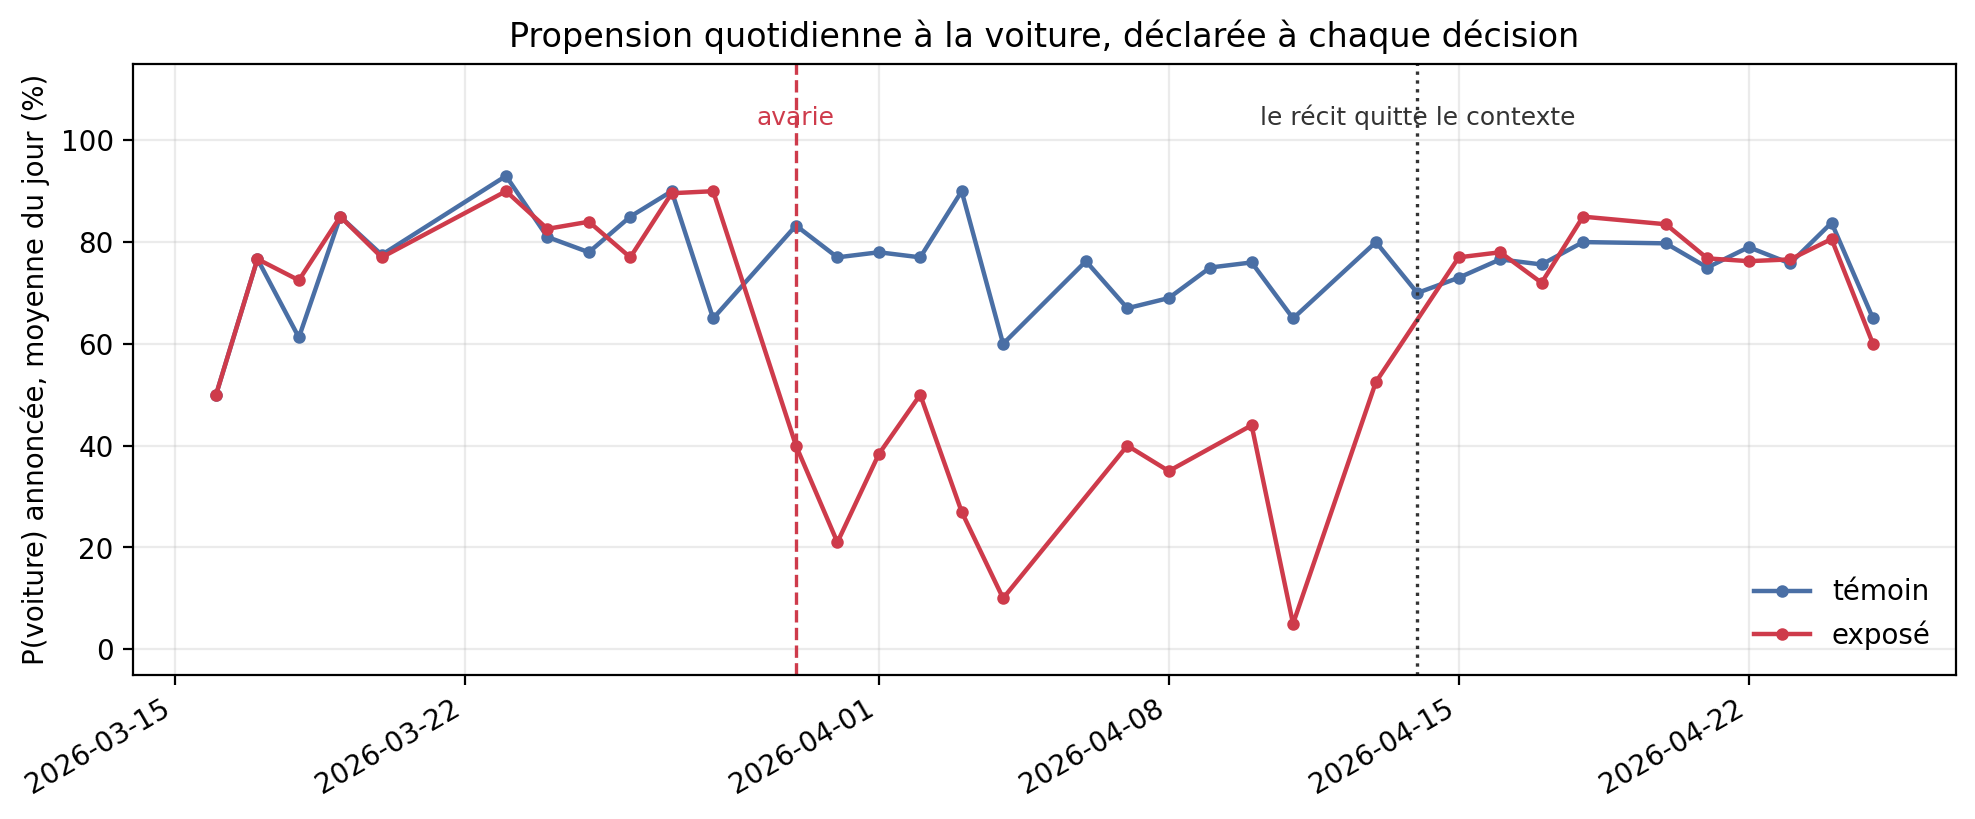
\includegraphics[width=\columnwidth]{images/ch7_propension_quotidienne.png}
  \caption{Probability the agent grants the car, averaged over the decisions of the day. The measurement is daily and cuts the simulation into no phase.}
  \Description{Two daily time series of the probability the agent assigns to the car, in percent, over about six weeks of simulated days. The exposed agent and the unexposed control run together above 65 percent until the breakdown, after which the exposed series collapses to between 5 and 52 percent for roughly a fortnight before rejoining the control band. A dashed vertical line marks the breakdown and a dotted one the day the account leaves the context.}
  \label{fig:propensity}
\end{figure}

The propensity falls on the very day of the breakdown, from 90\,\% the day before to 40\,\%, then swings between 5 and 52\,\%. It returns into the band of the unexposed agent, which never leaves 65 to 90\,\%, on 15 April. The account of the incident, for its part, disappears from the decision prompts after the 13th. One day separates these two dates, and neither is deduced from the service duration: the first is read on the announced probabilities, the second on the text actually sent to the model.

The agent took the car again twelve times during the period, and no contradiction of a belief was recorded: the belief born of the breakdown was not being served, so there was nothing to contradict. The extinction observed is therefore that of the memory wearing out, not that of a contradiction.

Declared opinions follow the same movement, then return to their earlier level. Asked outside any decision about six criteria, the exposed agent falls on five of them at the milestone that follows the breakdown: the safety of the car goes from 8 to 3, convenience from 9 to 6, comfort from 8 to 5, speed from 9 to 8 and cost from 6 to 5. At the two following milestones, all five have found their starting value again. The environment, which no incident of the device targets, stays at 3 across the four surveys. On the car, the unexposed agent moves on none of the six criteria.

\begin{figure*}[tp]
  \centering
  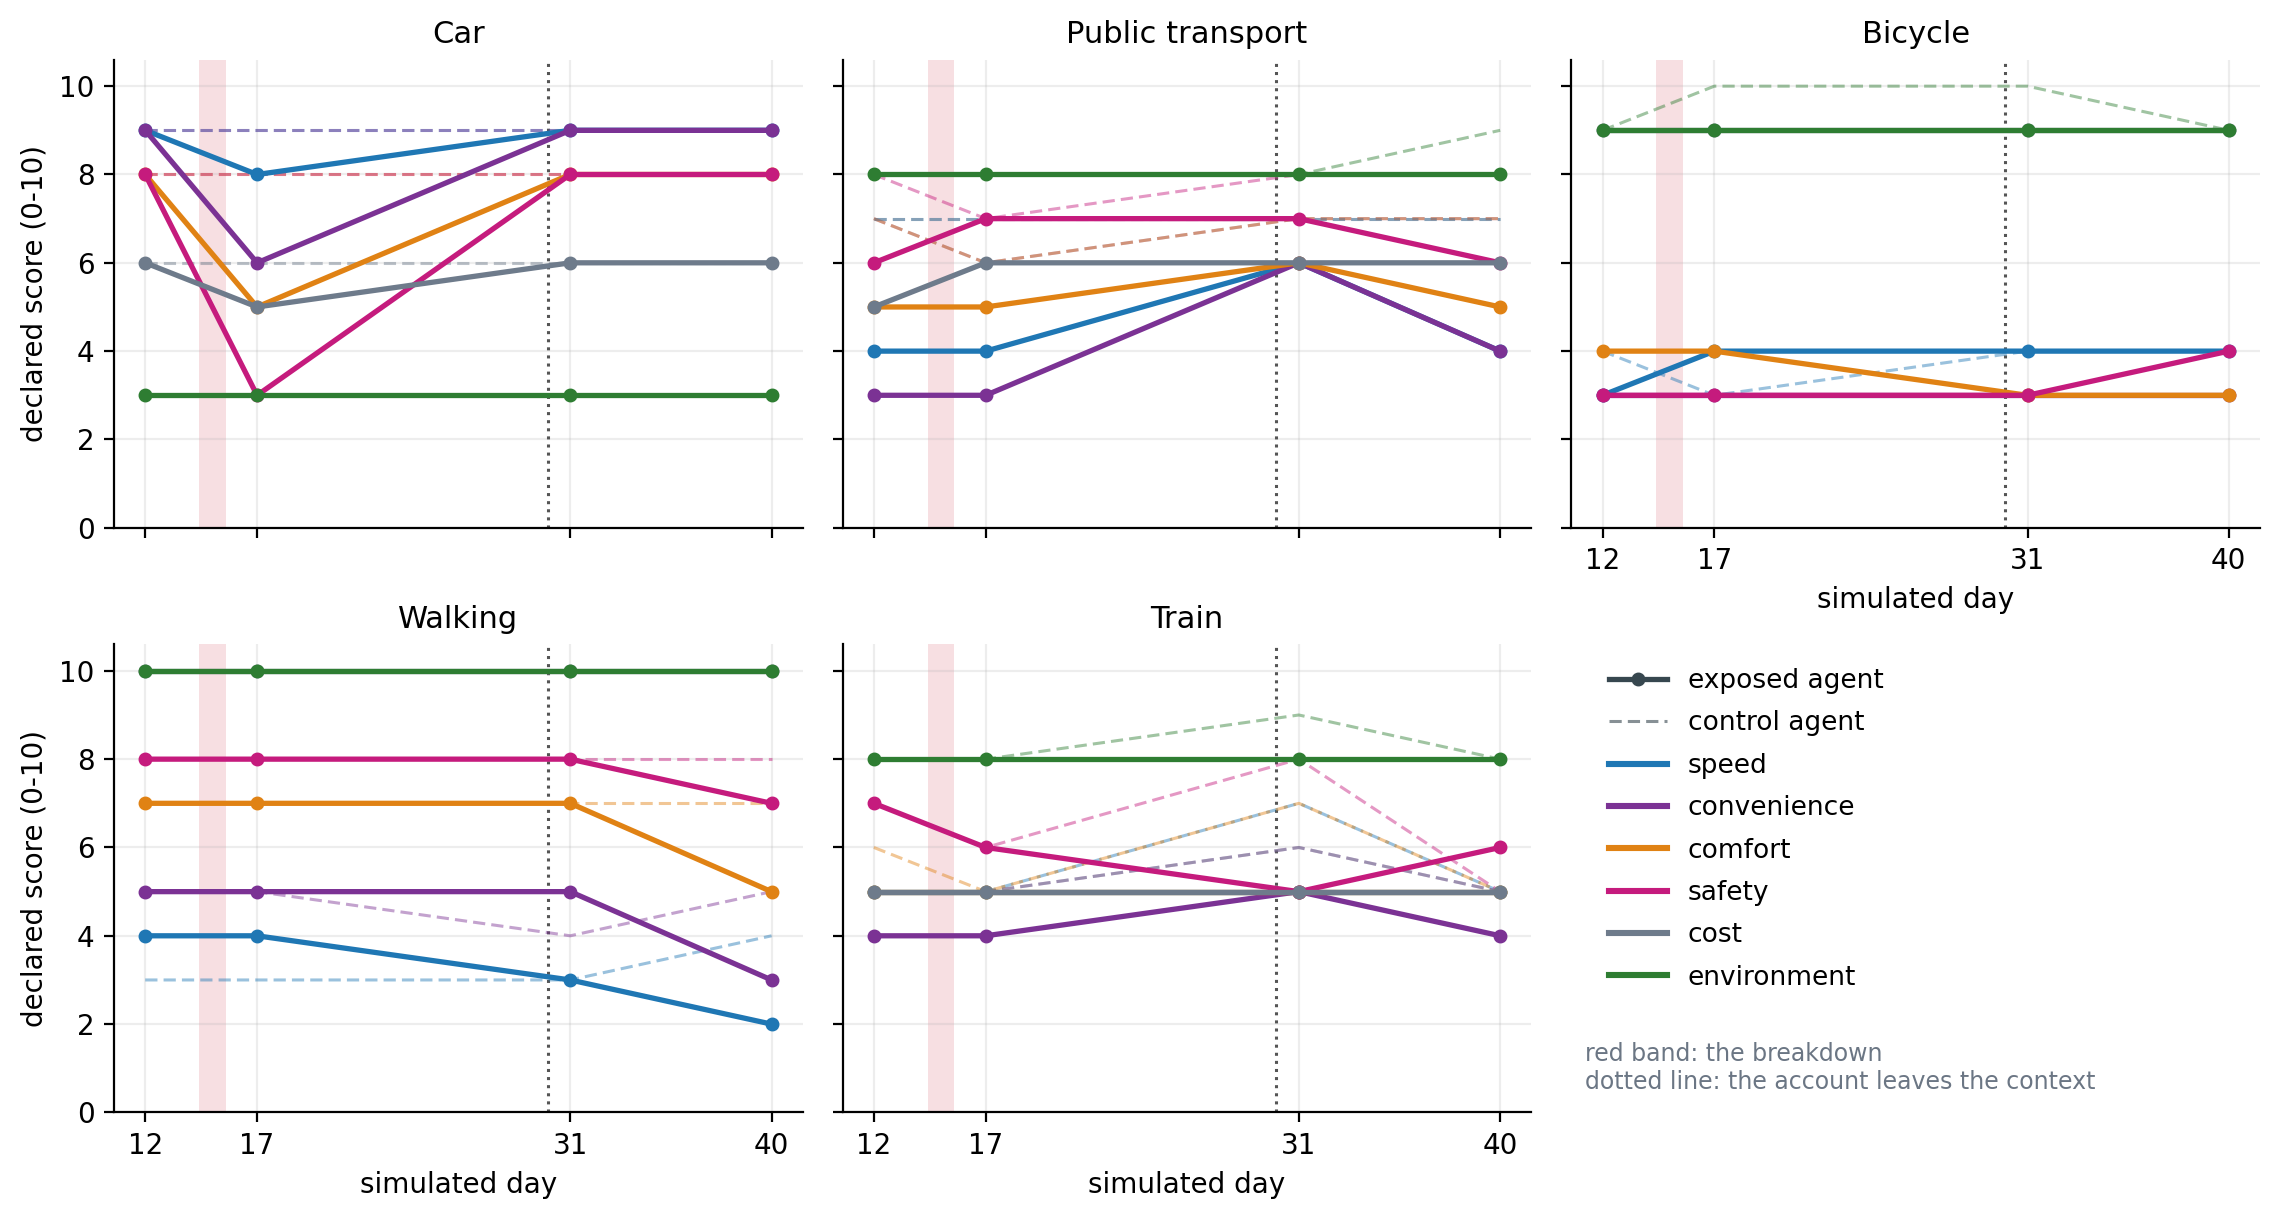
\includegraphics[width=\textwidth]{images/ch7_affinites_tous_modes.png}
  \caption{Declared opinions, six criteria per mode, exposed agent as a solid line and unexposed agent dashed. The red band marks the breakdown, the vertical line the day its account leaves the context. The environment serves as a control question.}
  \Description{Five small panels, one per transport mode, each plotting six declared scores from 0 to 10 at four survey milestones. In the car panel, five of the six criteria of the exposed agent drop sharply at the second milestone and return to their starting values at the third and fourth, while the control agent's lines stay flat. In the panels for public transport, bicycle, walking and train, both agents drift without any common pattern.}
  \label{fig:affinities}
\end{figure*}

Public transport, the bicycle, walking and the train offer no such reading. Both agents drift there from one milestone to the next, nineteen of the thirty series for the exposed agent, sixteen for the control, and the movements do not resemble each other from one arm to the other. The car is the only mode where the exposed agent moves and the control does not; that is what makes the gap attributable to the breakdown rather than to the noise of the survey. A return to the starting level on five scales describes an opinion regenerated from the persona as soon as the context stops carrying the incident.

\subsection{The article read, then told at home}
\label{sec:press}

\subsubsection{The five events}

Five articles taken from the Toulouse local press each act through one or more channels. Gusts of the Autan wind above 80\,km/h close the city's fenced parks and expose the bridges over the Garonne. A rumour of bedbugs on the fabric seats of the metro and buses leaves the technical offer intact and the credibility of the mode dented. An open-ended strike of refuse collectors makes the pavements of the inner centre impassable without changing their geometry in any way. The street parade of La Machine pedestrianises the centre in front of a dense crowd. The launch of electrically assisted V\'el\^oToulouse erases the gradient of the hillsides.

None of these five pieces of information has a column in a classical system, and adding one would be complex, and endless, each day bringing a new piece of news.

\subsubsection{The device}

The experiment is played on a few households, over several consecutive days, with memory on. One member per household receives the text in the morning, before their first decision. The articles appeared in French; the five texts are given translated.

\begin{table}[tp]
  \caption{The three conditions under which each press event is played. All three hold the agent and vary the text it receives.}
  \label{tab:conditions}
  \begin{tabular}{@{}llp{0.24\columnwidth}p{0.24\columnwidth}@{}}
    \toprule
    \# & Condition & What the decider receives & What the condition separates \\
    \midrule
    C1 & Agent, nominal day & no article & the reference level of the day \\
    C2 & Agent, raw article & the press text as it appeared & the total effect of the event \\
    C3 & Agent, control text & a news text with no plausible link to mode choice, of matched length, the same for all five events & the effect of the content from the effect of adding a text \\
    \bottomrule
  \end{tabular}
\end{table}

The control text is a natural-science dispatch, matched in length to each article to within half a percent to eight percent. A distant text and a Toulouse news item are not worth the same to someone who lives in the city, and the gap between C3 and C1 carries that reservation.

\subsubsection{Predictions and how they are measured}

For each of the five events and each of the four modes, the modal share must rise, fall, or not move. Those twenty signs are written before the first call to the model.

\begin{figure}[tp]
  \centering
  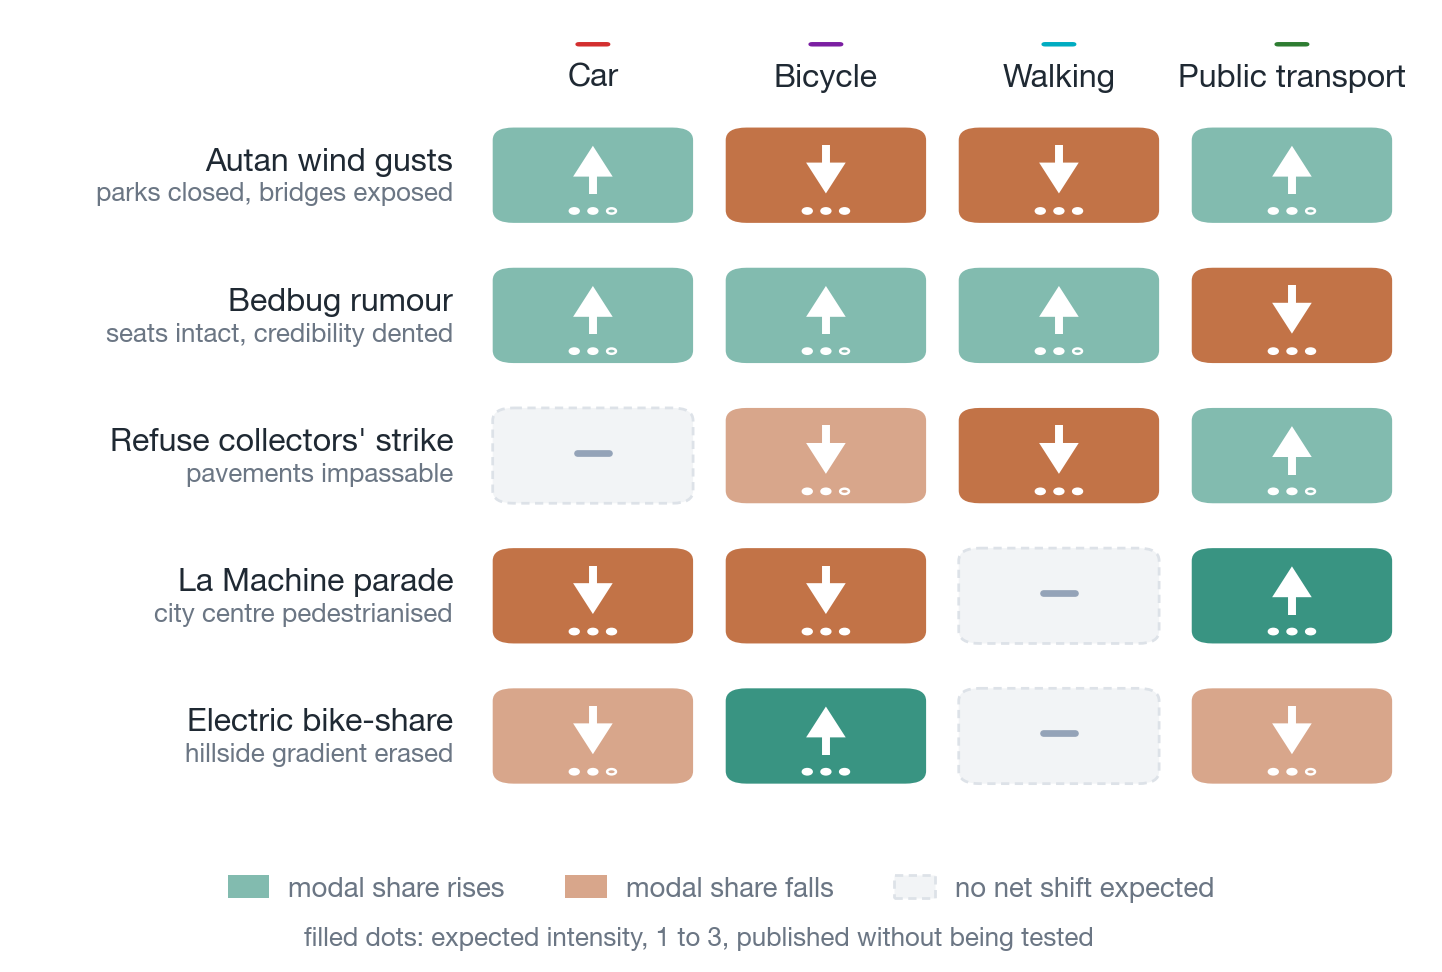
\includegraphics[width=\columnwidth]{images/ch7_grille_signes.png}
  \caption{The twenty expected signs, written before the first call to the model. Each cell carries the expected direction of the modal share shift under the raw article with respect to the nominal day, and its intensity as a number of dots. The three cells at zero are predictions of no net shift, which the measurement can refute as it would refute a reversed sign.}
  \Description{A grid of five rows, one per press event, by four columns, one per transport mode. Each of the twenty cells is coloured teal for an expected rise or clay for an expected fall, with an arrow pointing up or down and up to three filled dots for the expected intensity. Three cells are pale grey with a dashed border and a short horizontal dash, marking a prediction of no net shift.}
  \label{fig:signgrid}
\end{figure}

The rating the agent gives the article, on the scale of Section~\ref{sec:mechanism}, is set against this grid before it moves at all: it names the modes it judges affected and the direction of the effect. The gap between what it announces and what it does is a measurement in its own right, an agent that announces the right direction without moving having read the text without drawing any consequence from it.

The control text bounds the reading. It gives the amplitude of a modal shift with no relevant content, \todo{x.x | C3 $-$ C1} point, to be compared with the identical replay of the nominal day, which gives the decider's own noise.
